\chapter{Introduction (outline)}

\section{Amyloid: the field} % (fold)
% Organizational detail: AD and amyloid (which one should go first?). Center it on Amyloid, and then bring in AD as a central motivation for doing amyloid science.

% I think my focus should still be on Alzheimer's disease ... the practical purpose of my work is to understand how inositol works
% I am not trying to cure all amyloid diseases.

\subsection{Alzheimer's Disease}
% Here, my intention is to lead into the discussion of amyloid by giving a historical perspective and overview of AD
% And use AD as a motivation for why so much work has gone into studying amyloids.
\begin{outline}[enumerate]
\1 More than a hundred years have pass since Dr. Alois Alzheimer first presented the connection between the presence of neuronal plaques and the clinical symptoms of presenile dementia characteristic of Alzheimer's disease (AD).

\1 Today, AD is known to be the most common cause of dementia in persons of age 65 or older. With the increasing longevity of our population, AD is approaching epidemic proportions with no cures or preventative therapy available.\{Blennow,2006 \#221\}

% Elaborate on happened between the step above and the amyloid hypothesis?
\1 The discovery of amyloid plaque deposits of the brains of deceased dementia patients led to the formulation of the amyloid hypothesis which posits that amyloid aggregates may cause the pathogenesis of AD.  

\1 Decades after the initial discovery by Alois Alzheimer, A$\beta$, the central protein component of neuronal plaques, was synthetically produced in the laboratory. In vitro, A$\beta$ was found to precipitate out of solution almost immediately, which led to the discovery of A$\beta$ amyloid fibrils.

% \2 A$\beta$ is produced by intramembrane proteolytic cleavage of the larger amyloid-$\beta$ precursor protein (APP) by $\beta$-secretase, and is produced constitutively as part of the normal cellular metabolism.\{Selkoe, 2002 \#222\} Depending on the position of the cleavage, A$\beta$ peptides of lengths varying from 38 to 43 residues can be produced. However, the peptides spanning residues 1--40 (A$\beta$40) or 1--42 (A$\beta$42) are predominantly found AD-associated plaques.

\end{outline}

\section{Mechanism of amyloid formation and toxicity}
% In this section I will talk about how amyloid aggregation is thought to work. Introduce the thermodynamic model for understanding fibril formation. I will now broadly introduce to amyloid.  
\begin{outline}[enumerate]
\1 Although the initial studies of amyloid was motivated by attempts to understand the etiology of AD, amyloid science now have grown into its own field.

\1 Many diseases have been demonstrated to be linked with the presence of amyloid. Type II diabetes, Prions, Parkinsons, Huntington's disease etc.

\1 From studying AD and these neurodegenerative diseases, we were able to learn a lot about biophysics of the amyloid state.

  \2 It is now known that amyloid is many different species and fibril are formed from a pathway. Different forms. Monomers aggregate to form oligomers with different conformations, which exists in equilibrium.  Amyloid fibrils are the visible endpoint of peptide aggregation and has a $\beta$-sheet structure.
  \2 Nucleation-polymerization process. The formation of amyloid is characterized by a slow nucleation-phase, a rare event, followed by a more rapid growth phase (polymerization). Amyloid aggregation pathway. Monomers aggregate to form oligomers. There are different type of oligomers. Some are on-pathway to fibril formation. Some are found to be end-points of the aggregation pathway.
  \2 In the laboratory, scientists have been able to produce amyloid from a variety of proteins by denaturing them.

% Key question in the field: What is the toxic species?
\1 Toxicity. In recent years, focus has been on finding the relevant toxic species. Oligomers have been identified as a favorite for toxic causative agent.  One hypothesis is that they interact with cellular membranes and by doing so perturb the membranes, which leads to cell death.

% Understanding the toxicity or finding out whether there is a toxic species in part validates the amyloid hypothesis. 
\1 The structure of oligomers have been difficult to obtain via traditional experimental protein structural determination methods because many of the aggregates aren't soluble and are structurally disordered.   
  \2 The monomeric form and fibril forms are probably not toxic. It is most recently hypothesized that amyloid causes cellular toxicity by perturbing the cell membrane (making them ion-permeable).
  \2 Write a paragraph about amyloid formation and lipid membranes ?
\end{outline}


\section{Therapeutic options for amyloid diseases}
% Cure, method of prevention; is there hope?
% Here I will provide an overview of the different types of treatments from a drug perspective.
\begin{outline}
  \1 Briefly mention non-small molecule treatments.
  \1 And there is also inhibiting the formation of amyloid using small-molecule therapies ... I will focus on small-molecules.  Talk about why small molecules. 
\end{outline} 


\section{Mechanism of Amyloid inhibition by small molecules}
% Small molecules as a treatment option of AD and other amyloid diseases.  
  \begin{outline}[enumerate]
    \1 Amyloids are a attractive drug target.  Many small molecules are found to bind to amyloids and inhibit amyloid fibrils.   Small molecules may be one effective way to develop a treatment for amyloid disorders because they have the potential to be developed into drugs.
      % Here I can take a cue from Justin Lemkul`'s recent review paper.
      % Talk about the different kinds of small molecules that have been found to inhibition amyloid formation.  Here I will also provide a summary of what people know about the mechanism by which they inhibit amyloid formation.
      
      \2 Pharmacological perspective of the challenge of developing an Alzheimer's drug. In order to effectively treat Alzheimer's, requires small molecule to pass the blood brain barrier.  This is a difficult thing to achieve.

      \2 They share common chemical features.  All of them are planar in geometry, have aromatic rings, and polar functional groups around the edge of these aromatic rings.

      \2 Thioflavin T and Congo red are dye molecules which are used in identifying the presence of amyloid.  Both molecules bind to the fibrillar form of amyloids. They are also both found to inhibit fibril formation.
      
      \2 Polyphenols is a class of molecules which binds to one or species of amyloid. These molecule is found in green tea and wine.  They have anti-oxidative properties.
      
    \1 These molecules are found to be weak binders.  That is, they are non-specific binders and exert their effects at high concentrations.
      
        \2 Mechanism of action. Some small molecules inhibit fibril formation, some inhibits oligomerization. They are all found to be weak binders and act on millimolar concentrations. The strongest activity is a polyphenol EGCG.
\end{outline}


\section{Molecular Dynamics (MD) Simulations} % (fold)
% Motivate MD simulations
\1 Molecular dynamics simulations are a useful tool to study the structure, dynamics, and interaction of biomolecules. MD simulations employ an empirical mathematical function to describe the atomic interactions in a molecular system, and together with classical laws of Newtonian mechanics, atomic trajectories of motion are generated. Thermodynamic and kinetic properties can then be extracted as time averages from these trajectories and used to make a number of predictions that are often experimentally challenging to observe or measure. 
\1 MD simulation studies have been useful in studying many existing fundamental problems of biology and biochemistry, including protein dynamics and function, protein folding, biomolecular self-aggregation, and protein-ligand binding.
% Study protein dynamics - importance of protein dynamics.

\subsection{Methodological Details} % (fold)
% Describe the details of molecular dynamics simulations

% A set of numerical computation algorithm which solves numerically solves the N-body problem. Solves a system of Newton's equations of motion, and provides the time-trajectory of atoms with femtosecond time resolution. 

% The integration algorithm is XXX. Time steps used are typically 2 femtoseconds to capture the hydrogen bond vibrational motion. [MORE DETAILS AND EQUATIONS HERE] [Ref: Chris Madill's and Tom's thesis]
% Details of the mathematics (need to review the basic theory + Taylor series expansion) - get a book - tomorrow maybe?

% The assumption at a hand-wave level adapted from Tom's thesis

\1 Why is MD correct? (Some fundamental assumptions of MD)
  \2 The Born-Oppenheimer approximation: electronic and nuclear motions are uncoupled, and therefore can be treated separately. MD does not account for the movement of electrons. Although electrons are not taken into account in MD simulations, their presence is implicitly accounted for via the use of potential energy functions.  Atomic nuclei can be treated as classical particles.

  % \2 Review the basic derivations of MD simulation equations and why they work:
  %   \3 Assume a small integration step (why is 2 fs chosen it is both biological and for numerical stability purposes). Roughly MD follows these steps:
  %     \4 F = -grad E, where E is given by the force field potential energy function.
  %     \4 Determine acceleration for each atom from the forces on each atom
  %     \4 From acceleration determine momentum 
  %     \4 Determine positions

% - Relationship between force and energy 
% - Relationship between momentum and velocity 
% - Why numerical approach must be used (no analytical solution for N > 2)
% - How is the force field plugged into the general algorithm.

  \2 Application of an empirical force field can be used approximate atomic interactions in the system.
      \3 Include the general force field equation, where
      \[ V(R) = bonds + angles + impropers + dihedrals + pair interactions \]

      \3 There many different force fields (AMBER, Gromos etc), however, in this thesis we apply OPLS-AA force field in all of our simulations.
        \4 Many parameters that need to be determined. Often one approach is to fit to QM calculations.  Optimal to compute these for small compounds and adjust parameters by comparing calculations to experimental results.

% \1 Step to produce a molecular simulation:
%   \2 First take a structure from crystallography or NMR, or homology-modelling data.
%   \2 In the algorithm, the forces acting on each atom are estimated from [insert equation here]

\section{Role of molecular dynamics simulations in drug discovery}
\1 (Why computational?) Can help us get protein dynamics is important for understanding protein function. We want to understand protein function because we want to be able to design drugs to cure diseases.

\1 Cheaper, faster, get atomic resolution. Modelling can be used to rapidly prototype an experimental idea -- for example, one can easily "mutate" residues and test it out. In recent years structure-based computer modeling of protein-ligand interactions have become a core component of modern drug discovery. REF: Mobley, Dill 2004 Computers are advancing thus it is cheaper, MD may be used as a drug discovery platform. In terms of drug discovery, can be used to determine whether a chemical change will produce a more potent drug candidate.

% MD is more straightforward if there is a folded, protein structure.
\1 A broad application of simulations of proteins is to computationally design drugs and combining that with structure-based drug design.
  \2 First you solve a protein structure using conventional structural determination methods such as X-ray Crystallography or perhaps NMR.  Typically you would have an idea of where the binding pocket is as well. 
  \2 Then taking a protein force field and apply MD simulations to the protein structure in the presence of the putative ligand.  Because the binding affinity is very high (usually the binding specificity ...


\subsection{Application: Protein-ligand binding}
\1 A important application of MD simulation in biochemistry is the predicting of protein-ligand binding free energies.
  \2 
  \2 Absolute binding free energy
  \2 Relative binding free energy

\1 Have an X-ray crystal structure and know of a putative binding pocket. [See Tom's thesis]
\1 Ligands typically have high binding affinity to a binding pocket. So we want to find a high specificity binder for which ever protein that we are looking to inhibit.
  \2 Binding is a low probability event in simulations. Therefore it is infeasible to simulate using brute-force MD sampling.
  \2 Methods used to determine binding free energies using MD: 
  \3 Linear interaction energy - ???
  \3 MM/PBSA - no explicit account for solvents
  \3 Thermodynamic perturbation 
       \4 thermodynamic integration
       \4 free energy perturbation

\1 Protein-Ligand binding theory (independent of MD simulations)
% Below is a summary of an excerpt from Tom's thesis on structure-based drug discovery.
% Design of antibiotics 
% 1) Target determination (biochemical)
% 2) Structural determination (Xray, NMR, or homology); active site identified; Here would be useful to get the holo structure of the protein
% 3) Screen for inhibitors against a chemical library or in silico docking.

  \2 Currently state of the art computational binding studies take into the account of change in protein conformation.  An alternative technique, docking, where the binding affinity is measured without taking into account of the protein conformational entropy, is computational cheaper, but inaccurate for identifying true drug candidates.  However, it may work well in a screen step.

  \2 Enzyme and the ligand must bind tightly and specifically, so to avoid large drug doses to inhibit the enzyme, which may have adverse side effects (toxicity) in the human body.

  \2 Binding constant is a measure of the affinity of a ligand to a protein. It is the concentration at which 50\% of the drug is bound to the protein. In experimental studies, Kd is often used to identify potential binders. Typically in a classical biochemistry sense/setting, the higher lower the dissociation constant of a drug, the more effective the drug is likely to be.
    \3 Equation: Equilibrium protein+ligand <-> (protein-ligand)aq

  \2 Experimental techniques for determining Kd - which experimental techniques can be used to gain an estimate of binding affinity?
   \3 Look this up ... I have no clue.  Might be nice to know.

  \2 Amyloid inhibition in the framework of tradition enzyme inhibition mechanism

    \3 Can we think about amyloid inhibition as a standard protein-ligand binding problem? Not really.We have the exact opposite of this framework with amyloids. Most inhibitors are found to be very weak binders ... how are they working as a drug then? And how do we approach this with MD simulations?

    \3 The enzyme and ligand inhibition / binding model cannot be directly applied to understanding amyloid inhibition.  No folded structure, no putative structure (there are many, which one?), no putative binding site (generally presents a surface).

    \3 In AD, there is the added challenge of the drug being able to cross the brain barrier, while remaining non-neurotoxic.  What kind of drugs cross the BBB?  Typically hydrophobic drugs.
    
\subsection{Application of MD simulations to amyloid inhibition}
MD studies using brute-force sampling. Aid in medicinal chemistry by making suggestions for how to design new AD drugs

\subsubsection{Review of MD studies of amyloid inhibition by small molecules}
%  Excerpt from Transfer proposal
\1 In recent years, molecular dynamics simulations have been intensively used to investigate the molecular basis of the structure and stability of amyloid fibrils. However, most of these studies were focused on A$\beta$ and large A$\beta$ aggregates,\{Fawzi, 2008 \#553;Esposito, 2008 \#567;Sgourakis, 2007 \#609;Wei, 2006 \#656;Tarus, 2006 \#628 Karsai, 2006 \#658\} and thus, were computationally limited by the complexity of the molecular systems. To date, few studies have attempted to provide statistically meaningful results pertaining to general mechanisms of protein self-aggregation and amyloid formation. Furthermore, despite the abundance of MD studies of A$\beta$, few studies have systematically examined the mechanism of action of small molecule inhibitors of amyloids. MD simulations of Congo red binding have only been done with the protofibril-like crystal structure composed of the segment GNNQQNY.\{Wu, 2007 \#621\} A recent simulation study of an N-methylated peptide with A$\beta$16--22 models of amyloid aggregates has provided insight into the possible mechanism of action of peptide inhibitors of amyloid formation.\{Soto, 2007 \#597\} This peptide inhibitor was shown to preferentially bind monomers to form dimers, possibly acting to inhibit fibril formation by sequestering monomers. However, peptide-based inhibitors have poor pharmacological profiles as they are actively broken down by proteases in the stomach and are difficult to transport across the blood-brain barrier. In addition, these peptide inhibitors specifically target A$\beta$ and thus do not have the potential to treat multiple amyloid diseases.

\subsubsection{Molecular mechanism of binding of dye molecules}
% Review of what is known about dye binding on amyloid fibrils.
Two types of binding modes. Bind flat on amyloid surface. Interact with hydrophobic groups exposed on the amyloid fibrils.
Doesn't explain why the dye molecules are also able to suppress fibril formation.

% Can the birefringence be explained by these binding modes?

\section{Challenges of MD}
\1 There are challenges to MD on both the length and time scale. Biology happens on the time scale of milliseconds, hours, days and years. With simulation we only get microseconds at most.  And we still need really big computers to make stuff happen at the millisecond timescale, and they are not continuous simulations. See: Anton by DE Shaw. 

\1 We don't know the accuracy of our empirical force fields. We don't have effective ways to determine whether our simulations are converged.

\section{Challenges of understanding amyloid inhibition}
% Here describe how I designed my study to navigate the challenges presented by the amyloid inhibition problem and MD simulations - rationale
% At this point, explain and discuss my approach, study-design and rationale. Include the matrix figure.

% Figure~\ref{fig:}

\section{Thesis objectives and rationale}
\begin{figure}
  \centering
  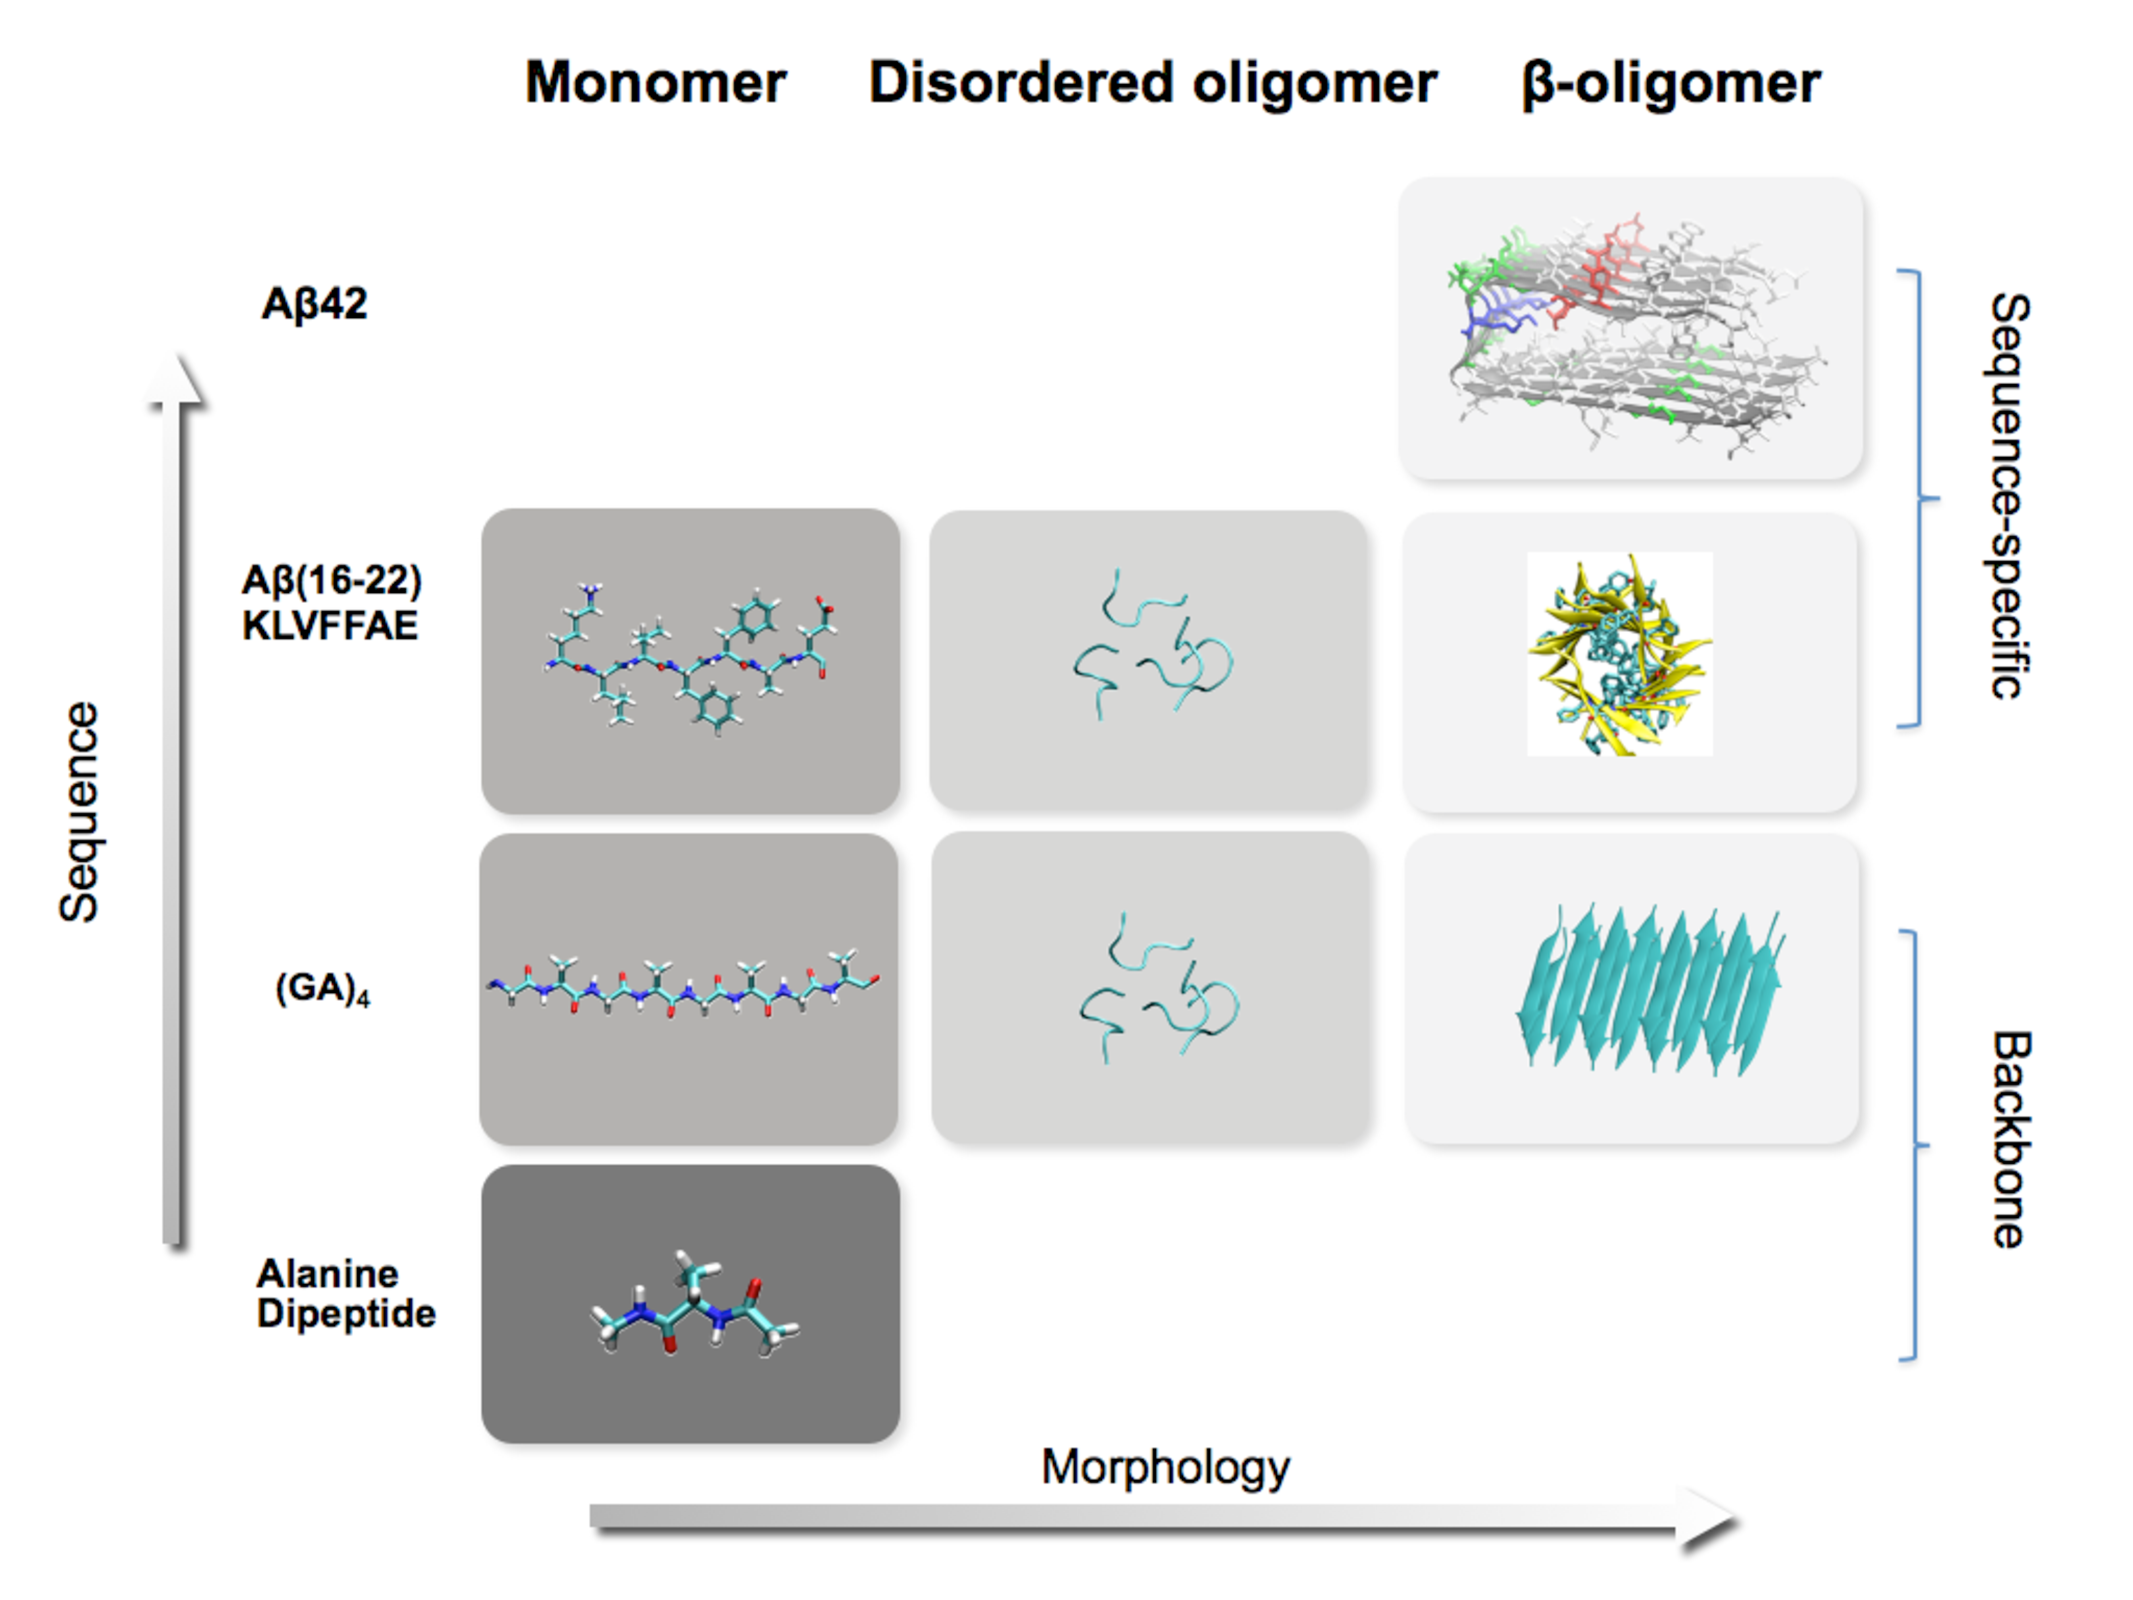
\includegraphics[width=6in]{figures/introduction/matrix.pdf}
  \caption[Rationale]{Shows the progression from small, model systems to larger and structurally more complex systems involving the full-length A$\beta$42 peptide.}
  \label{fig:rationale}
\end{figure}

\1 A$\beta$ peptides are completely disordered.  Because A$\beta$ amyloid formation consists of many different types of aggregates, a single conformation cannot be assumed for binding.  We also do not know what the binding site looks like, where it is located on these structures.

\1 Beginning with the simplest model systems for an amyloidogenic peptide, the alanine dipeptide, we systematically examine binding of inositol with systems of both increasing sequence and structural complexity.

% Use brute force simulations
\1 We exploit conventional MD simulation techniques because we can't readily pick a reaction coordinate as in tradition enzyme-ligand binding problems. Using large-scale sampling and repeats of many simulations to determine the binding mechanism and binding equilibria.

% section thesis_objectives_and_rationale (end)


%%%%%%%%%%%%%%%%%%%%%%%%%%%%
% Molecular simulation notes
%%%%%%%%%%%%%%%%%%%%%%%%%%%%
% Why MD?
% To properly understand drug binding - we need motion!

% The first thing that want to talk about is why people have used molecular dynamics to study proteins.  Think about the reader ... they should not have questions like ... why can't you just use docking, pick a single structure -- no single structure.  Can't assume binding sites!  

% Why couldn't you have just taken A$\beta$42 and simulated that from the beginning, why model peptides?  Because computationally infeasible?  -- Why ?  I think the answer comes down to answering in part why computing protein folding is hard.

% Is MD is just pretty pictures or can we get quantities that are experimentally comparable.  Are some of these things experimentally testible?  -- what are some things that I've tried to compute in my simulations that others haven't been able to do? This will be something that I should anticipate and be ready to address at my defense.  In sum, all the stuff that ever came up at my student seminar and my committee meetings ... I should be ready to answer.

% Talk about how MD has been used in the past and present.

% Thesis organization notes:
% KEY results:
% 
% Sugar binding modes 
% 
% Binding cooperativity
% 
% Binding at the surface, grooves 
% 
% Have not explained whether the inositol is an kinetic or thermodynamic inhibitor - speculate that it's kinetic 
% 
% Have not resolved whether Scyllo and chiro both work or does not work on KLVFFAE
%     - Scyllo has more specific binding modes. TODO: peel back the densities for Scyllo and chiro and see the binding hotspots. Do they differ and how ?
%     - Scyllo can stabilize oligomers of KLVFFAE.  Chiro not sure yet. 

% Should I put this here ? As advised by Sarah: If I can

% \section{Significance of thesis}

% - most complete study done on a single amyloid inhibitor 
% 
% - detection of sugar binding modes from molecular simulations 
% 
% - we have demonstrated that simulations are useful for studying weak binding 
%    - generally useful method for studying sugar binding modes to proteins 
% 
% - design of next generation of amyloid inhibitors for Alzheimer's disease 
% 
%    - selection targeting to the KLVFFAE face!!!! 
%          - both Joanne and Mark said tonnes of literature supporting this face is relevant for inhibition!!!
%           - so far Scyllo best at binding to this face!! This is an interesting conclusion / difference that thus only could tell from from the abeta42 model because it has two different faces which brought out the preferential binding of Scyllo to this face. 
% 
%            - Regis what if we used Epi or myo a positive control .... Which would make this binding to the KLVFFAE face of abeta42  hypothesis more compelling ... If another inhibitor which worked in vitro also preferentially bound to the KLVFFAE face.


% Introduction from transfer proposal:
% 
% In AD, the amyloid fibrils that form the extracellular plaques are a result of the self-aggregation of monomeric A$\beta$ peptides. A variety of structural studies using electron microscopy (EM), X-ray diffraction, and solid-state NMR spectroscopy (SSNMR) have demonstrated that the core of A$\beta$ fibrils contains a cross-$\beta$ sheet structure.\{Sunde, 1997 \#226;Petkova, 2002 \#205\} Furthermore, amyloid fibrils exhibit green birefringence upon binding to Congo red and enhanced fluorescence upon binding to Thioflavin T. High resolution data from SSNMR revealed that both A$\beta$40 and A$\beta$42 fibrils are highly ordered in-register parallel $\beta$-sheets.\{Tycko, 2004 \#194\} Although there is evidence that A$\beta$40 and A$\beta$42 aggregate and form fibrils through distinct pathways,\{Bitan, 2003 \#280\} the SSNMR and EM data show no discernable structural differences between the two.\{Tycko, 2004 \#194\}
% 
% In addition to AD, amyloid fibril formation also plays a pathologically-relevant role in many other diseases, such as type 2 diabetes, Parkinson's disease, and Huntington's disease.\{Chiti, 2006\#51\} Many different proteins, including some that are not involved in
% disease, have also been found to form amyloid fibrils \emph{invitro.}\{Chiti, 2006 \#51\} Recently, atomic-level structures of amyloid
% fibrils of hexameric peptide segments from 14 different amyloidogenic proteins have been determined using X-ray microcrystallography.\{Sawaya, 2007 \#233\} These structures all share a common motif of two tightly interdigitated $\beta$-sheets stacked together with a water-excluding interface.
% 
% A long standing question is which aggregate species is responsible for neurotoxicity. Although fibrils have been long thought to be the primary neurotoxic species, the poor quantitative correlation of plaque presence with disease severity has made fibril-related neurotoxicity difficult to explain.\{Haass, 2007 \#3\} More recently, experimental evidence has shown that the levels of soluble A$\beta$ fibrillation intermediates correlate well with neural dysfunction, and that these species are more neurotoxic than mature fibrils,\{Caughey, 2003 \#277;Lambert, 1998 \#278;Hoshi, 2003 \#279\} suggesting that they may play an important role in AD pathogenesis.
% 
% EM and atomic force microscopy (AFM) experiments of soluble A$\beta$ prefibrillar assemblies have found them to be annular, spherical, or curvilinear in shape. Protofibrils, in particular, are curvilinear, filamentous structures that are smaller than mature fibrils and are approximately 5--10 nm in diameter.\{Haass, 2007 \#3\} Furthermore, protofibrils bind to dyes Thioflavin T (ThT) and Congo Red (CR), suggesting the presence of substantial $\beta$-sheet content.\{Walsh, 2007 \#2;Haass, 2007 \#3;Harper, 1999 \#319;Kodali, 2007 \#367\} Despite the importance of these prefibrillar species in causing neurodegeneration, their molecular structures are still not known. However, a recent SSNMR study demonstrated that a late stage, neurotoxic A$\beta$40 spherical intermediate contained fibril-like $\beta$-sheet structure.\{Chimon, 2007\#415\}
% 
% 
% Currently, no available treatments for AD can prevent or stop the progression of the disease. One promising therapeutic approach is the development of small-molecule inhibitors of A$\beta$ aggregation.\{LeVine, 2007 \#432\} Recently, \emph{scyllo}-inositol, one of eight stereoisomers of a class of simple polyols, has emerged as a therapeutic candidate.\{McLaurin, 2006 \#513\} The four most common stereoisomers of inositol in nature are \emph{scyllo}-, \emph{myo}-, \emph{epi}-, and \emph{chiro}-inositol.\{Fisher, 2002 \#541\} Both \emph{scyllo}- and \emph{myo}-inositol are found in high concentrations in the human brain. \emph{Myo}-inositol is the most abundant isomer and is found in high concentrations in tissues of the central nervous system (CNS), serving both as a precursor for inositol lipid synthesis and as a physiologically important osmolyte.\{Fisher, 2002 \#541\} \emph{Scyllo}-, \emph{myo}-, and \emph{epi}-, but not \emph{chiro}-inositol, have been shown to inhibit A$\beta$42 fibril assembly, stabilize an oligomeric complex of A$\beta$42, and attenuate A$\beta$-oligomer-induced neurotoxicity \emph{in vitro.}\{McLaurin, 2000 \#536\} Moreover, inositol exhibits stereochemistry-specific effects on A$\beta$ fibril inhibition and cytotoxicity: \emph{scyllo}- and \emph{epi}- are more effective than \emph{myo}-inositol, whereas \emph{chiro}-inositol has no activity.
% 
% \emph{In vivo} studies with a transgenic mouse model of AD demonstrated that alleviation of symptoms after inositol treatment was correlated with a decrease in the levels of soluble A$\beta$ oligomers, suggesting that the beneficial effects of \emph{scyllo}-inositol may be attributed to the inhibition and/or disaggregation of high-order A$\beta$ oligomers.\{McLaurin, 2006 \#513\} Taken together, these results suggest that \emph{scyllo}-inositol, and possibily its derivatives, are a potential therapy for AD with the ability to change the course of the disease. \emph{Scyllo}-inositol is currently in phase two of clinical trials.

% The mechanism of action of inositol is not known at the molecular level. Amyloid fibrillation is a multi-stage process involving different species at each stage. Small molecule inhibitors such as inositol may interact with species at various stages of aggregation. Due to the heterogeneous and non-crystalline nature of prefibrillar species, experimental determination of the molecular structures of these amyloid species remains a challenge. However, computer simulations are not limited by these experimental challenges and can provide the atomistic level of detail needed to elucidate the action of inositol on the inhibition of amyloid formation.

% \section{Molecular Dynamics Simulations}
% 
% Molecular dynamics simulations are a useful tool to study the structure, dynamics, and interaction of biomolecules. MD simulations employ an empirical mathematical function to describe the atomic interactions in a molecular system, and together with classical laws of Newtonian mechanics, atomic trajectories of motion are generated. Thermodynamic and kinetic properties can then be extracted as time averages from these trajectories and used to make a number of predictions that are often experimentally challenging to observe or measure. MD simulation studies have been useful in studying many existing fundamental problems of biology and biochemistry, including protein folding, biomolecular self-aggregation, and protein-ligand binding.
% 
% In recent years, molecular dynamics simulations have been intensively used to investigate the molecular basis of the structure and stability of amyloid fibrils. However, most of these studies were focused on A$\beta$ and large A$\beta$ aggregates,\{Fawzi, 2008 \#553;Esposito, 2008 \#567;Sgourakis, 2007 \#609;Wei, 2006 \#656;Tarus, 2006 \#628 Karsai, 2006 \#658\} and thus, were computationally limited by the complexity of the molecular systems. To date, few studies have attempted to provide statistically meaningful results pertaining to general mechanisms of protein self-aggregation and amyloid formation. Furthermore, despite the abundance of MD studies of A$\beta$, few studies have systematically examined the mechanism of action of small molecule inhibitors of amyloids. MD simulations of Congo red binding have only been done with the protofibril-like crystal structure composed of the segment GNNQQNY.\{Wu, 2007 \#621\} A recent simulation study of an N-methylated peptide with A$\beta$16--22 models of amyloid aggregates has provided insight into the possible mechanism of action of peptide inhibitors of amyloid formation.\{Soto, 2007 \#597\} This peptide inhibitor was shown to preferentially bind monomers to form dimers, possibly acting to inhibit fibril formation by sequestering monomers. However, peptide-based inhibitors have poor pharmacological profiles as they are actively broken down by proteases in the stomach and are difficult to transport across the blood-brain barrier. In addition, these peptide inhibitors specifically target A$\beta$ and thus do not have the potential to treat multiple amyloid diseases. 

% Here, we propose to use MD to perform a systematic study of the molecular mechanism of action of inositol, a promising therapeutic candidate for the treatment of AD.


